\section{Multidimensional Integrals} %

% --- COUNTER SETUP FOR THIS SECTION ---
\newcounter{savedSecMulti}
\newcounter{savedThmMulti}

One powerful way to understand the Riemann integral of a function $f: A \to \mathbb{R}$ in higher dimensions is to view it as calculating the volume \textit{under} the graph of the function. The script formalizes this using the concept of a \qt{hypograph}, which your TA sketched in the notes as the volume trapped above a domain $A$.

% --- SCRIPT JUMP (13.40) ---
\setcounter{savedSecMulti}{\value{section}}
\setcounter{savedThmMulti}{\value{theorem}}
\setcounter{section}{13}
\setcounter{theorem}{39} 

\begin{definition}[Hypograph]
Let $A \subset \mathbb{R}^n$ and $f : A \to [0, \infty)$. The \textbf{hypograph} of $f$ is defined as the set
\[
\Gamma_A(f) := \{ (x, y) \in \mathbb{R}^n \times \mathbb{R} \mid x \in A, 0 \le y < f(x) \} \subset \mathbb{R}^{n+1}.
\]
\end{definition}

% RESTORE COUNTERS
\setcounter{section}{\value{savedSecMulti}}
\setcounter{theorem}{\value{savedThmMulti}}
% --------------------------

\begin{extra}
\textbf{Gemini 3.1's Note: What is a Hypograph?}\\
Don't let the Greek prefix intimidate you! \qt{Hypo} just means \qt{under} (like hypothermia means under-heating). In Calc 1, when you integrated $f(x)$ from $a$ to $b$, you were finding the 2D area \textit{under} the curve. The hypograph is literally just that geometric shape: the region trapped between the floor ($z=0$) and the ceiling ($z=f(x,y)$). 
\end{extra}

% --- GEMINI VISUALIZATION 1: THE HYPOGRAPH ---
\begin{center}
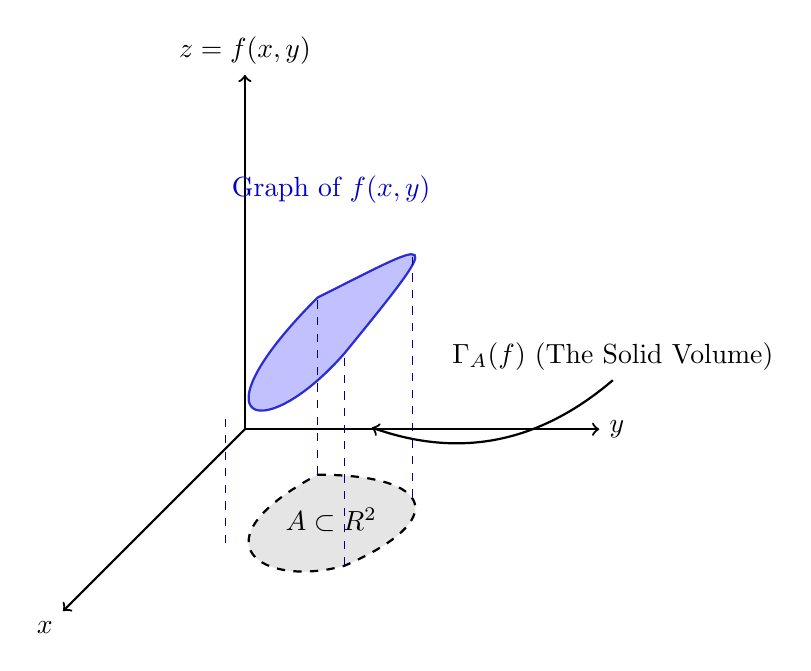
\begin{tikzpicture}[scale=1.5, text=black]
    % 3D Axes
    \draw[->, thick] (0,0,0) -- (3,0,0) node[right] {$y$};
    \draw[->, thick] (0,0,0) -- (0,3,0) node[above] {$z = f(x,y)$};
    \draw[->, thick] (0,0,0) -- (0,0,4) node[below left] {$x$};
    
    % Domain A in the xy-plane (z=0)
    \draw[fill=gray!20, draw=black, thick, dashed] 
        (1,0,1) .. controls (2,0,1) and (2.5,0,2) .. 
        (2,0,3) .. controls (1.5,0,3.5) and (0.5,0,2.5) .. 
        (1,0,1) -- cycle;
    \node at (1.5, 0, 2) {$A \subset \mathbb{R}^2$};
    
    % The Surface (Ceiling)
    \draw[fill=blue!30, opacity=0.8, draw=blue!80!black, thick] 
        (1,1.5,1) .. controls (2,2,1) and (2.5,2.5,2) .. 
        (2,1.8,3) .. controls (1.5,1.2,3.5) and (0.5,1.0,2.5) .. 
        (1,1.5,1) -- cycle;
        
    % Connecting lines (walls of the hypograph)
    \draw[dashed, blue!50!black] (1,0,1) -- (1,1.5,1);
    \draw[dashed, blue!50!black] (2,0,1.5) -- (2,2.05,1.5);
    \draw[dashed, blue!50!black] (2,0,3) -- (2,1.8,3);
    \draw[dashed, blue!50!black] (0.8,0,2.5) -- (0.8,1.05,2.5);
    
    \node[blue!80!black] at (1.5, 2.8, 2) {Graph of $f(x,y)$};
    \node at (3.5, 1, 1) {$\Gamma_A(f)$ (The Solid Volume)};
    
    % Arrow pointing to the volume
    \draw[->, thick, shorten >=2pt] (3.5, 0.8, 1) to[bend left] (1.8, 0.8, 2);
\end{tikzpicture}
\end{center}
% ---------------------------------------------

% --- SCRIPT JUMP (13.42 & 13.43) ---
\setcounter{savedSecMulti}{\value{section}}
\setcounter{savedThmMulti}{\value{theorem}}
\setcounter{section}{13}
\setcounter{theorem}{41} % Skipping 13.41 to land exactly on 13.42

\begin{lemma}[Riemann Integral as Jordan Measure]
Let $A \subset \mathbb{R}^n$ be a set. A function $f: A \to [0, \infty)$ is Riemann integrable if and only if the hypograph $\Gamma_A(f)$ is Jordan measurable in $\mathbb{R}^{n+1}$. In such a case,
\[
\int_A f = \mu_{n+1}(\Gamma_A(f)).
\]
\end{lemma}

\begin{corollary}[Integrability of Continuous Functions]
Suppose that $E \subset \mathbb{R}^n$ is a Jordan measurable set and $f : \overline{E} \to [0, \infty)$ is a continuous function. Then, $f$ is Riemann integrable over $E$.
\end{corollary}

% RESTORE COUNTERS
\setcounter{section}{\value{savedSecMulti}}
\setcounter{theorem}{\value{savedThmMulti}}
% --------------------------

\noindent
\textbf{TA's Survival Rule:} Thanks to Corollary 13.43, in practice, nonnegative continuous functions are almost always integrable on nicely behaved (Jordan measurable) closed sets!


\subsection{Normal Domains and Fubini's Theorem}

Defining the integral via the hypograph is mathematically rigorous, but it doesn't help us actually calculate a number. To compute multidimensional integrals, we need to slice the domain into standard 1D integrals. We do this using \textbf{Normal Domains}.

\begin{definition*}[Normal Domains / Projectable Regions]
There are two primary ways to slice a 2D region $A \subset \mathbb{R}^2$:
\begin{enumerate}
    \item \textbf{Type I (x-normal):} The domain is bounded left/right by constants $a, b$, and top/bottom by functions of $x$:
    \[
    A = \{ (x, y) \in \mathbb{R}^2 \mid a \le x \le b, \text{ and } g_1(x) \le y \le g_2(x) \}
    \]
    \item \textbf{Type II (y-normal):} The domain is bounded bottom/top by constants $c, d$, and left/right by functions of $y$:
    \[
    A = \{ (x, y) \in \mathbb{R}^2 \mid c \le y \le d, \text{ and } h_1(y) \le x \le h_2(y) \}
    \]
\end{enumerate}
\end{definition*}

% --- GEMINI VISUALIZATION 2 & 3: NORMAL DOMAINS ---
\begin{center}
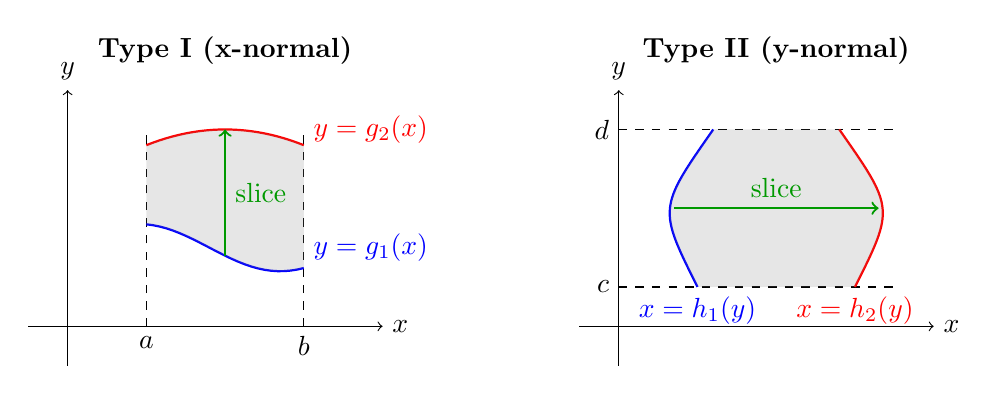
\begin{tikzpicture}[scale=1.0]
    
    % LEFT PANEL: Type I
    \begin{scope}[xshift=0cm]
        \node at (2, 3.5) {\textbf{Type I (x-normal)}};
        % Axes
        \draw[->] (-0.5, 0) -- (4, 0) node[right] {$x$};
        \draw[->] (0, -0.5) -- (0, 3) node[above] {$y$};
        
        % Constants a, b
        \draw[dashed] (1, 0) node[below] {$a$} -- (1, 2.5);
        \draw[dashed] (3, 0) node[below] {$b$} -- (3, 2.5);
        
        % Curves
        \draw[thick, blue, domain=1:3] plot (\x, {0.3*sin(\x*100) + 1}); % g1
        \draw[thick, red, domain=1:3] plot (\x, {-0.2*(\x-2)*(\x-2) + 2.5}); % g2
        
        % Labels
        \node[blue, right] at (3, 1) {$y = g_1(x)$};
        \node[red, right] at (3, 2.5) {$y = g_2(x)$};
        
        % Shading
        \fill[gray, opacity=0.2, domain=1:3] (1, {0.3*sin(1*100) + 1}) -- plot (\x, {-0.2*(\x-2)*(\x-2) + 2.5}) -- (3, {0.3*sin(3*100) + 1}) -- plot[domain=3:1] (\x, {0.3*sin(\x*100) + 1}) -- cycle;
        
        % Slicing arrow (Vertical)
        \draw[->, thick, green!60!black] (2, {0.3*sin(2*100) + 1}) -- (2, {-0.2*(2-2)*(2-2) + 2.5}) node[midway, right] {slice};
    \end{scope}

    % RIGHT PANEL: Type II
    \begin{scope}[xshift=7cm]
        \node at (2, 3.5) {\textbf{Type II (y-normal)}};
        % Axes
        \draw[->] (-0.5, 0) -- (4, 0) node[right] {$x$};
        \draw[->] (0, -0.5) -- (0, 3) node[above] {$y$};
        
        % Constants c, d
        \draw[dashed] (0, 0.5) node[left] {$c$} -- (3.5, 0.5);
        \draw[dashed] (0, 2.5) node[left] {$d$} -- (3.5, 2.5);
        
        % Curves (x as function of y)
        \draw[thick, blue] (1, 0.5) .. controls (0.5, 1.5) .. (1.2, 2.5); % h1
        \draw[thick, red] (3, 0.5) .. controls (3.5, 1.5) .. (2.8, 2.5); % h2
        
        % Labels
        \node[blue, below] at (1, 0.5) {$x = h_1(y)$};
        \node[red, below] at (3, 0.5) {$x = h_2(y)$};
        
        % Shading
        \fill[gray, opacity=0.2] (1, 0.5) .. controls (0.5, 1.5) .. (1.2, 2.5) -- (2.8, 2.5) .. controls (3.5, 1.5) .. (3, 0.5) -- cycle;
        
        % Slicing arrow (Horizontal)
        \draw[->, thick, green!60!black] (0.7, 1.5) -- (3.3, 1.5) node[midway, above] {slice};
    \end{scope}

\end{tikzpicture}
\end{center}
% --------------------------------------------------------

\begin{theorem*}[Fubini's Theorem for Normal Domains]
Let $A \subset \mathbb{R}^2$ be a normal domain with respect to the x-axis (Type I). If $f : A \to \mathbb{R}$ is continuous, the double integral can be evaluated as an iterated integral:
\[
\iint_A f(x, y) \, dA = \int_a^b \left[ \int_{g_1(x)}^{g_2(x)} f(x, y) \, dy \right] dx.
\]
If $A$ is Type II, we switch the order: integrate $dx$ first, then $dy$ on the outside.
\end{theorem*}

\begin{extra}
\textbf{Gemini 3.1's Note: The \qt{Loaf of Bread} Method}\\
Fubini's theorem is the absolute backbone of Calculus 2 computations. If the integral is asking for the volume of a loaf of bread, Fubini says: 
\begin{enumerate}
    \item First, pick a specific spot along the crust ($x$).
    \item Slice the bread vertically there, and find the area of that one 2D slice (the inner integral $\int dy$).
    \item Add up all the 2D slices from the front of the loaf to the back (the outer integral $\int dx$).
\end{enumerate}
\textbf{Golden Rule of Fubini:} The outermost integral bounds \textbf{must always be constants!} If you end up with variables in your final evaluation step, you've mixed up your order!
\end{extra}

% --- GEMINI VISUALIZATION 4: LOAF OF BREAD (FUBINI) ---
\begin{center}
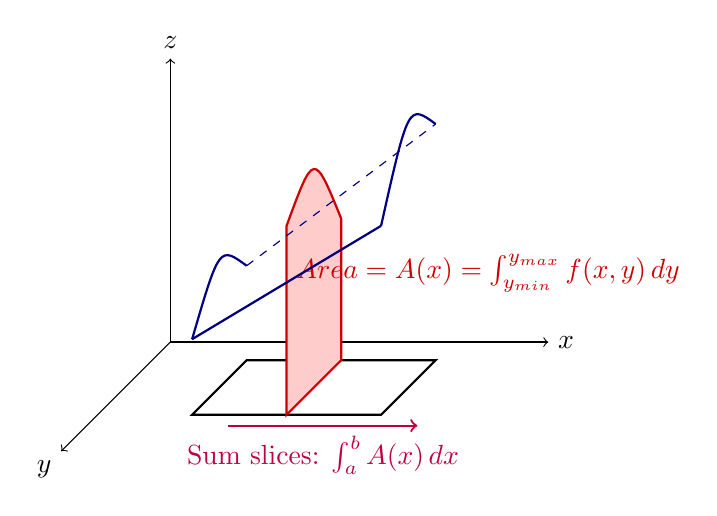
\begin{tikzpicture}[scale=1.2, text=black]
    % Axes
    \draw[->] (0,0,0) -- (4,0,0) node[right] {$x$};
    \draw[->] (0,0,0) -- (0,3,0) node[above] {$z$};
    \draw[->] (0,0,0) -- (0,0,3) node[below left] {$y$};
    
    % The Loaf Base (x from 1 to 3, y from 0.5 to 2)
    \draw[thick] (1,0,0.5) -- (3,0,0.5) -- (3,0,2) -- (1,0,2) -- cycle;
    
    % A generic slice at x_0 = 2
    \draw[fill=red!20, draw=red!80!black, thick] (2,0,0.5) -- (2,0,2) -- (2,2,2) .. controls (2,2.5,1.25) .. (2,1.5,0.5) -- cycle;
    
    % Annotate the slice
    \node[red!80!black, right] at (2, 1.5, 2) {$Area = A(x) = \int_{y_{min}}^{y_{max}} f(x,y) \, dy$};
    
    % Draw the rest of the loaf (outline)
    \draw[thick, blue!50!black] (1,1,0.5) .. controls (1,1.5,1.25) .. (1,0.8,2); % Back slice top
    \draw[thick, blue!50!black] (3,2.5,0.5) .. controls (3,3.0,1.25) .. (3,2.0,2); % Front slice top
    
    % Connect the loaf
    \draw[dashed, blue!50!black] (1,1,0.5) -- (3,2.5,0.5);
    \draw[thick, blue!50!black] (1,0.8,2) -- (3,2.0,2);
    
    % Add integration arrow
    \draw[->, thick, purple] (1, -0.5, 1) -- (3, -0.5, 1) node[midway, below] {Sum slices: $\int_a^b A(x) \, dx$};
\end{tikzpicture}
\end{center}
% ------------------------------------------------------


\subsection{Gemini 3.1's Extra Practice Examples}

To truly master this, we need to do the math. Here are 4 classic exams-style examples showing exactly how to set up and execute these integrals.

\begin{example}[Type I Normal Domain: The Triangle]
Evaluate $\iint_A 2xy \, dA$, where $A$ is the triangle bounded by the x-axis ($y=0$), the line $y=x$, and the vertical line $x=1$.

\textbf{Step 1: Understand the Domain.} 
This is a perfect Type I domain. The x-values go from $a=0$ to $b=1$. For any fixed $x$, the y-values go from the floor ($y=0$) up to the ceiling ($y=x$). 

\textbf{Step 2: Set up Fubini and Integrate.}
\begin{align*}
\iint_A 2xy \, dA &= \int_0^1 \left( \int_0^x 2xy \, dy \right) dx \\
&= \int_0^1 \left[ xy^2 \right]_{y=0}^{y=x} dx \\
&= \int_0^1 (x(x)^2 - x(0)^2) \, dx \\
&= \int_0^1 x^3 \, dx \\
&= \left[ \frac{1}{4}x^4 \right]_0^1 = \frac{1}{4}.
\end{align*}
\end{example}


\begin{example}[The Classic \qt{Switching Bounds} Trap]
Evaluate the integral: 
\[
I = \int_0^1 \int_y^1 e^{x^2} \, dx \, dy
\]
\textbf{The Problem:} If you try to integrate $e^{x^2}$ with respect to $x$, you will get stuck immediately. It has no elementary antiderivative! 

\textbf{The Solution:} We must switch the order of integration. But we \textbf{cannot} just blindly swap the bounds to $\int_y^1 \int_0^1$. We have to redraw the domain.

% --- GEMINI VISUALIZATION 5: SWITCHING BOUNDS ---
\begin{center}
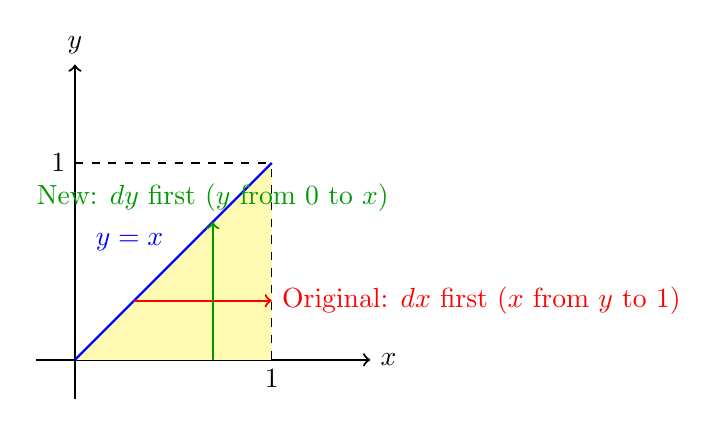
\begin{tikzpicture}[scale=2.5]
    % Axes
    \draw[->, thick] (-0.2, 0) -- (1.5, 0) node[right] {$x$};
    \draw[->, thick] (0, -0.2) -- (0, 1.5) node[above] {$y$};
    
    % The Domain
    \fill[yellow!30] (0,0) -- (1,0) -- (1,1) -- cycle;
    \draw[thick, blue] (0,0) -- (1,1) node[midway, above left] {$y=x$};
    \draw[dashed] (1,0) node[below] {$1$} -- (1,1);
    \draw[dashed] (0,1) node[left] {$1$} -- (1,1);
    
    % Original Slicing (Horizontal / dx dy)
    \draw[->, thick, red] (0.3, 0.3) -- (1.0, 0.3) node[right] {Original: $dx$ first ($x$ from $y$ to $1$)};
    
    % New Slicing (Vertical / dy dx)
    \draw[->, thick, green!60!black] (0.7, 0) -- (0.7, 0.7) node[above] {New: $dy$ first ($y$ from $0$ to $x$)};
\end{tikzpicture}
\end{center}
% ------------------------------------------------

By looking at the diagram, if we want to integrate with respect to $y$ first (vertical slices), the y-bounds go from the floor ($y=0$) to the slanted roof ($y=x$). The outer x-bounds are constants from $0$ to $1$. 

\begin{align*}
I &= \int_0^1 \left( \int_0^x e^{x^2} \, dy \right) dx \\
&= \int_0^1 \left[ y e^{x^2} \right]_{y=0}^{y=x} dx \\
&= \int_0^1 x e^{x^2} \, dx
\end{align*}
Now, this is an easy Calc 1 substitution! Let $u = x^2$, so $du = 2x \, dx$, meaning $x \, dx = \frac{1}{2}du$.
\[
I = \int_0^1 \frac{1}{2} e^u \, du = \frac{1}{2}(e^1 - e^0) = \frac{1}{2}(e - 1).
\]
\end{example}


\begin{example}[Triple Integrals and 3D Volumes]
Find the volume of the solid tetrahedron bounded by the coordinate planes ($x=0, y=0, z=0$) and the plane $x + y + z = 1$.

% --- GEMINI VISUALIZATION 6: THE TETRAHEDRON ---
\begin{center}
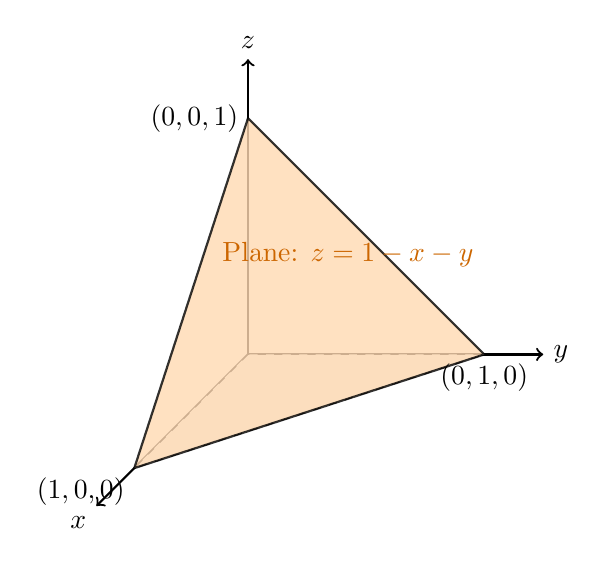
\begin{tikzpicture}[scale=2.5]
    % 3D Axes
    \draw[->, thick] (0,0,0) -- (1.5,0,0) node[right] {$y$};
    \draw[->, thick] (0,0,0) -- (0,1.5,0) node[above] {$z$};
    \draw[->, thick] (0,0,0) -- (0,0,2) node[below left] {$x$};
    
    % Vertices of the tetrahedron
    \coordinate (X) at (0,0,1.5); % (1,0,0) in our custom projection
    \coordinate (Y) at (1.2,0,0); % (0,1,0)
    \coordinate (Z) at (0,1.2,0); % (0,0,1)
    
    % Draw back faces dashed
    \draw[dashed, fill=gray!10] (0,0,0) -- (X) -- (Y) -- cycle; % xy plane floor
    \draw[dashed] (0,0,0) -- (Z);
    
    % Draw the slanted front face
    \draw[thick, fill=orange!30, opacity=0.8] (X) -- (Y) -- (Z) -- cycle;
    
    % Labels
    \node[left] at (Z) {$(0,0,1)$};
    \node[below] at (Y) {$(0,1,0)$};
    \node[below left] at (X) {$(1,0,0)$};
    
    \node[orange!80!black] at (0.7, 0.7, 0.5) {Plane: $z = 1 - x - y$};
\end{tikzpicture}
\end{center}
% -----------------------------------------------

\textbf{Step 1: Set the bounds.}
\begin{itemize}
    \item \textbf{Inner (z):} Travels from the floor ($z=0$) to the slanted roof ($z = 1 - x - y$).
    \item \textbf{Middle (y):} Look down at the shadow on the xy-plane. It's a triangle bounded by $y=0$ and the line $x+y=1 \implies y = 1 - x$.
    \item \textbf{Outer (x):} The absolute constants on the x-axis are from $x=0$ to $x=1$.
\end{itemize}

\textbf{Step 2: Integrate.}
\begin{align*}
\text{Volume} &= \int_0^1 \int_0^{1-x} \int_0^{1-x-y} 1 \, dz \, dy \, dx \\
&= \int_0^1 \int_0^{1-x} (1 - x - y) \, dy \, dx \\
&= \int_0^1 \left[ (1-x)y - \frac{1}{2}y^2 \right]_0^{1-x} dx \\
&= \int_0^1 \left( (1-x)(1-x) - \frac{1}{2}(1-x)^2 \right) dx \\
&= \int_0^1 \frac{1}{2}(1-x)^2 \, dx \\
&= \left[ -\frac{1}{6}(1-x)^3 \right]_0^1 = -\frac{1}{6}(0) - \left(-\frac{1}{6}(1)\right) = \frac{1}{6}.
\end{align*}
\end{example}